\newlecture{1}{Hello, \LaTeX}

\section{Getting Started}

\subsection{What is \LaTeX}

\begin{frame}{What is \LaTeX}
	\begin{block}{From Wikipedia, the free encyclopedia\footnotemark[1]}
		\LaTeX\ (lah-tekh, lah-tek or lay-tek, a shortening of Lamport \TeX) is a document preparation system. When writing, the writer uses plain text in markup tagging conventions to define the general structure of a document (such as \structure{article}, \structure{book}, and \structure{letter}), to stylize text throughout a document (such as \textbf{bold} and \textit{italic}), and to add citations\footnotemark[1] and cross-references. \medskip
		
		A \TeX\ distribution such as \TeX Live or Mik\TeX\ is used to produce an output file (such as PDF or DVI) suitable for printing or digital distribution. \medskip
		
		Within the typesetting system, its name is stylized as \LaTeX.	
	\end{block}
	
	\footnotetext[1]{\LaTeX\ - \url{https://en.wikipedia.org/wiki/Latex}}

\end{frame}

\begin{frame}{A brief History of \TeX\ and \LaTeX}
	Donald Kunuth from Stanford University is the specialist in programming art. In year 1977, he had just received his first samples from the new typesetting system of the publisher's, and its quality was so far below that of the first edition of Volume 2 that he couldn't stand it. Kunuth decided to implement a mathematical composition system by himself (since he is a computer scientist). He figured that this would take about 6 months (Ultimately, it took nearly 10 years). The system is named as \TeX, of both the meaning of Greek letters $\tau\epsilon\chi$, and ``technical ''. \medskip
	
	\LaTeX\ was created in 1983 by Leslie Lamport, when he was working at SRI. He needed to write \TeX\ macros for his own use, and thought with a little extra effort he could make a general package usable by others. Then \LaTeX\  developed rapidly and now there are thousands of packages written in \TeX\ macros available for direct usage.
	
\end{frame}

\subsection{Distributions and IDEs}

\begin{frame}{Installation of \LaTeX}
	Though there are some other distributions of \LaTeX (like Mik\TeX), \TeX Live is recommended in this lecture.
	\begin{block}{Windows \& Linux}
		Download \TeX Live on the \href{https://mirrors.tuna.tsinghua.edu.cn/}{tuna mirrors}
		\smallskip
				
		\small{\url{https://mirrors.tuna.tsinghua.edu.cn/CTAN/systems/texlive/Images/}}
	\end{block}
	\begin{block}{MacOS}
		Download Mac\TeX\ on the \href{https://mirrors.tuna.tsinghua.edu.cn/}{tuna mirrors}		
		\smallskip
		
		\small{\url{https://mirrors.tuna.tsinghua.edu.cn/CTAN/systems/mac/mactex/}}
	\end{block}
	\begin{block}{Linux (Debian/Ubuntu)}
		Enter the command (fast with apt source mirror) 
		\smallskip
		
		\mintinline{shell}|sudo apt-get install texlive-full|
	\end{block}
\end{frame}

\begin{frame}{Selection of IDEs}
	There are various IDEs recommended that support \LaTeX , for example
	\begin{block}{Texmaker}
		\url{http://www.xm1math.net/texmaker/}
	\end{block}
	 
	\begin{block}{Sublime Text}
		\url{http://www.sublimetext.com/}
	\end{block}
	Follow the instructions on \url{https://www.zhihu.com/question/36038602}
	
	\begin{block}{Visual Studio Code}
		\url{https://code.visualstudio.com/}
	\end{block}
	Follow the instructions on \url{https://zhuanlan.zhihu.com/p/38178015}
	\bigskip
	
	They all have cross-platform support for Windows, Linux and MacOS.
\end{frame}

\begin{frame}{Write \LaTeX\ on Overleaf (Online)}
	Another alternative choice is to write \LaTeX\ online with the technology of \href{https://www.overleaf.com/}{Overleaf}. It's free for personal usage and supports share editing which is very useful in group work.
	\begin{figure}
	\centering
	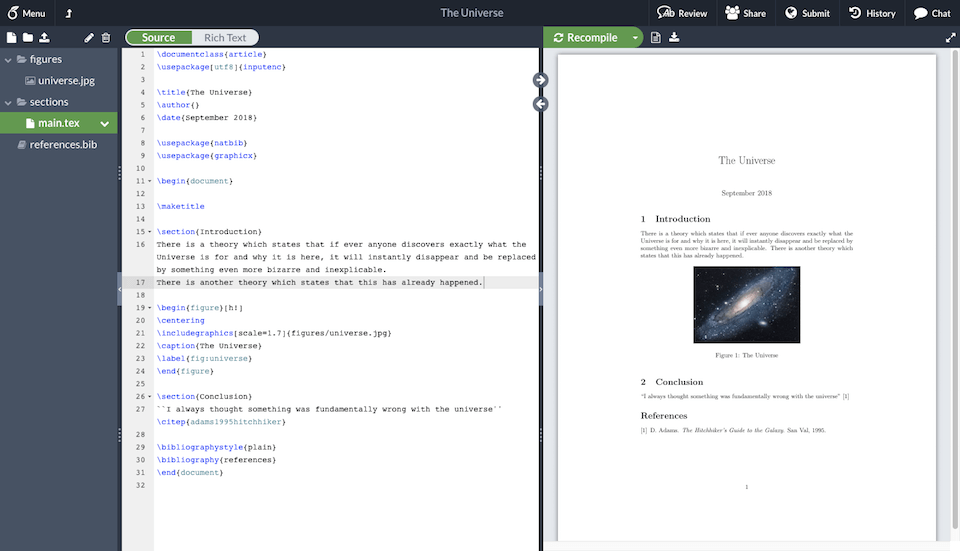
\includegraphics[width=0.7\linewidth]{../overleaf.png}
	\caption{Layout of the Overleaf Online \LaTeX\ Editor.}
	\end{figure}
\end{frame}

\subsection{Documentation}

\begin{frame}[fragile]{Documentation of \LaTeX}

	If you've installed a full version of \TeX Live (as strongly recommended), the full \LaTeX\ documentation is already on your computer. \medskip
	
	Open the command line and input the command 
	
\begin{command}
\begin{minted}{shell}
texdoc <docname>
\end{minted}
\end{command}
		
	You can also use the online version on \urllink{http://www.texdoc.net/} \medskip
	
	For example, you can use the following types for the \structure{docname}
	\begin{description}
		\item[tex] 		about \structure{\TeX}
		\item[article] 	about documentclass \packagename{article}
		\item[beamer] 	about documentclass \packagename{beamer} (used to create slides)
		\item[pgf]		about packages \packagename{tikz} and \packagename{pgf} (used to draw graphs)
	\end{description}
	\smallskip
	Try to \alert{texdoc} about all new things and then you'll be an expert in \LaTeX.
\end{frame}

\section{Layout of a Document}

\subsection{A Simple Document}

\begin{frame}[fragile]{A Simple Document}

	A typical (simplest) \LaTeX\ example is presented here.
	\begin{example}
		\inputminted{latex}{../examples/simple.tex}
	\end{example}
	Code started with \LC|\| is called a \structure{command}, and a pair of \LC|\begin{}| and \LC|\begin{}| is called an \structure{environment}.
\end{frame}

\subsection{Document Classes}

\begin{frame}[fragile]{All Begins with \packagename{documentclass}}
	\begin{definition}
		In a \LaTeX\ file, the \structure{first} line must be \\
		\LC|\documentclass[options]{class}|
	\end{definition}
	For example, you can use the following types for the \structure{class}
	\begin{description}
		\item[ariticle]	Write a report or an science article
		\item[report] 	Write a report
		\item[beamer]	Produce a lecture silde like this!
	\end{description}
	Some options can be added, for example, a typical case can be
	\mintinline{latex}|\documentclass[11pt,twoside,a4paper]{article}| \medskip
	
	Some details about the \structure{article} class will be introduced on the next page. More features about other classes and options can be found in the \LaTeX\ Document on your own.
\end{frame}

\begin{frame}[fragile]{The \packagename{article} Class}
	The \packagename{article} class is one of the most basic class in \LaTeX, it provides you with some normalized structure and format for report writing. So usually you will use the following command as the first line of your tex document:
	\mintinline{latex}|\documentclass[options]{article}| \medskip
	
	Some of the options values are listed below (the default values are \alert{alerted})
	\begin{itemize}
		\item \alert{\texttt{10pt}}, \packagename{11pt}, \packagename{12pt} or other sizes - the font size of the document
		\item \packagename{a4paper}, \packagename{a5paper}, \alert{\texttt{letterpaper}} - the size of paper
		\item \packagename{fleqn} - make the math equations left aligned (default middle aligned)
		\item \packagename{leqno} - display the serial numbers of math equations on the left (default on the right)
		\item \packagename{titlepage}, \alert{\texttt{notitlepage}} - whether to make the title an entire page
		\item \alert{\texttt{onecolumn}}, \packagename{twocolumn} - the number of columns of the document
		\item \packagename{twoside}, \alert{\texttt{oneside}} - influence the position of something on the page
	\end{itemize}
\end{frame}

\begin{frame}{Other classes}
	This project is open sourced and you can read the source code \urllink{https://github.com/SJTU-UMJI-Tech/LaTeX} to learn much (I promise) about the \packagename{beamer} class and some very interesting features of \LaTeX\ itself. There may also be a lecture about the \packagename{beamer} class in the future. \medskip

	When writing a \alert{long} report, \packagename{report} class can be used to provide some more layers of document (such as \packagename{chapter}) and different type settings. It's very similar to the \packagename{article} class, so it won't be specified. \medskip

	There are some other document classes such as \packagename{minimal}, \packagename{book}, \packagename{letter} and etc., but I think you may never use them.

\end{frame}

\subsection{The Preamble}

\begin{frame}[fragile]{The Preamble of a Document}

As in the simple example of a document, you should notice that there is a pair of
\begin{command}
\begin{LCL}
\begin{document}
  % some contents
\end{document}
\end{LCL}
\end{command}

This is called the \structure{body} of the document, and everything before the \structure{body}, including the \LC|\documentclass| line, is called the \structure{preamble} of the document. \medskip

In the preamble, you define the type of document you are writing and the language, load extra packages you will need, and set several parameters. For instance, a simplified document of the example above preamble would look like this:

\begin{example}
\begin{LCL}
\documentclass[a4paper]{article}
\title{A simple \LaTeX\ document}
\author{XX XXX}
\date{\today}
\end{LCL}
\end{example}

\end{frame}

\begin{frame}[fragile]{Title, Author and Date}
	It's very useful to generate a title on the first page of a document, in order to achieve it, these commands should first be added in the \structure{preamble}.
	\begin{example}
		\begin{minted}{latex}
\title{title}
\author{author name}
\date{\today}
		\end{minted}
	\end{example}
	You can simply use \mintinline{latex}{\date{\today}} to display your system date now.\\[0.5em]
	Then in the \structure{body} (will be introduced in the next section), use the command \LC{\maketitle} to generate the title, or title page if you added the option \packagename{titlepage} in the \LC|\documentclass|.
\end{frame}

\begin{frame}[fragile]{Magic of Packages}
	\LaTeX\ is a macro-based language, where most of useful commands are not built-in commands. These commands are defined in various packages, which should be included in the \structure{preamble}.
	\begin{command}
		\LC|\usepackage[options]{package}|
	\end{command}
	There are some very useful packages that you may \alert{ALWAYS} include:
	\begin{description}
		\item[\packagename{amsmath}] Define various maths environments
		\item[\packagename{amssymb}] Define various maths symbols
		\item[\packagename{geometry}] Adjust the margin, paper size, and etc.
		\item[\packagename{enumitem}] Generate a list like this!
		\item[\packagename{graphicx}] Insert images of all types
	\end{description}
	The usages of these and more packages will be introduced further.
\end{frame}

\begin{frame}[fragile]
	\frametitle{Common Packages}
	Here I provide a list of commonly used packages, you can start from using them after the lecture. \medskip

	\inputminted{latex}{../examples/packages.tex}
\end{frame}



%\begin{frame}
%	\frametitle{Geometry package}
%	The settings of the layout of the pages is in \structure{geometry} package.
%	\begin{command}
%		\samplecommand{usepackage}\{geometry\}\\
%		\samplecommand{geometry}\{\structure{options}\}
%	\end{command}
%	Some of the \structure{options} are listed below:
%	\begin{itemize}
%		\item \structure{paper} - same as the paper settings in documentclass
%		\item \structure{layout} - use another type of paper's layout
%		\item \structure{left/right} - the blank length on the left/right
%		\item \structure{top/bottom} - the blank length on the top/bottom
%	\end{itemize}
%	\begin{example}
%		\samplecommand{geometry}\{paper=a4paper,layout=a5paper\}
%		\samplecommand{geometry}\{left=2.5cm,right=2.5cm,top=2.5cm,bottom=2.5cm\}
%	\end{example}
%\end{frame}

\subsection{Document Body}
\begin{frame}[fragile]{Main Body of Document}
	The main body of your document which starts with \mintinline{latex}{\begin{document}} and ends with \mintinline{latex}{\end{document}} can be also called the \packagename{document} environment. All of the contents you'd like to display should be in it, and it \alert{MUST} be \alert{unique} in the whole file.
	\begin{example}
		\begin{minted}{latex}
\begin{document}
    \maketitle
    \newpage   %start the following contents in a new page
    \tableofcontents %automatically generate a table of content
    \newpage
    Hello, \LaTeX !
    % TODO: Add more contents
    ...
\end{document}
		\end{minted}
	\end{example}
	The position and order of title page and table of contents can be arbitrary, and there can be multiple table of contents in one document.
\end{frame}

\begin{frame}[fragile]{The \packagename{abstract} Environment}

When you are writing a paper, an \packagename{abstract} is often necessary in the beginning of the document.

\begin{latexexample}
\begin{abstract}
  This is a lecture about how to getting start in \LaTeX!
\end{abstract}
\end{latexexample}

The styling of the \packagename{abstract} will be based on the \packagename{documentclass} you are using. The example shows an \packagename{abstract} in the \packagename{beamer} class, which will be slightly different from that in the \packagename{article} class.

\end{frame}

\begin{frame}[fragile]{Comments}

As in other programming languages, comments are useful when you want to make your code readable. Adding a \LC|%| can make the whole line after it into a comment.

\begin{example}
\LC|% This is a comment|
\end{example} 

If you need multiline comments, use the \packagename{comment} environment provided by the \packagename{comment} package. (Add \LC|\usepackage{comment}| to your preamble.)

\begin{example}
\begin{LCL}
\begin{comment}
 some comments
 some other comments
\end{comment}
\end{LCL}
\end{example} 

\end{frame}

\begin{frame}[fragile]

Note that in the compiling, anything after a \LC|%| 
is omitted, including the newline character, so there is no space between ``comment'' and ``no'' in the second line.

\begin{latexexample}
A line
with space between ``line'' and ``with''

A line ended with comment% comments
no space between ``comment'' and ``no''
\end{latexexample}

PS: One newline, or any number of space and tab characters are usually considered as a single ``spacing'' in \LaTeX\ compilers. Two or more continuous newlines will cause a line break. We'll discuss it later in the lecture.


\end{frame}

\subsection{Document Sections}


\begin{frame}[fragile]{Sections}

Commands to organize a document vary depending on the document type, the simplest form of organization is the sectioning, available in all formats.

	\begin{command}
		\begin{multicols}{2}
			\begin{minted}{latex}
\section{name}
\subsection{name}
\subsection{name}
			\end{minted}
			\begin{minted}{latex}
\section*{name}
\subsection*{name}
\subsection*{name}
			\end{minted}
		\end{multicols}
		\vspace{-0.5em}
	\end{command}
	The default style (can be changed with \LC|\renewcommand| ) of sections is like \smallskip
	
	\structure{1 Example Section Name} 
	
	\structure{1.1 Example Subsection Name} 
	
	\structure{1.1.1 Example Subsubsection Name} \medskip
	
	If an asterisk (\structure{*}) is added, the sequence number will be hidden, and it won't be added to the table of contents. \medskip
	
	Note: (Sub)sections are \packagename{commands}, and the whole contents between two (sub)sections is belonged to the former (sub)section.
\end{frame}

\begin{frame}[fragile]
	\frametitle{Other Structures - Chapter, Part and Paragraph}
	\begin{command}
		\begin{multicols}{2}
			\begin{minted}{latex}
\chapter{name}
\part{name}
\paragraph{name}
\subparagraph{name}
			\end{minted}
			\begin{minted}{latex}
\chapter*{name}
\part*{name}
\paragraph*{name}
\subparagraph*{name}
			\end{minted}
		\end{multicols}
		\vspace{-0.5em}
	\end{command}
	In document classes such as \packagename{report} and \packagename{book}, some outer structures of \packagename{section} (\LC{\chapter} and \LC{\part}) can be used. \\[0.5em]
	\LC{\paragraph} and \LC{\subparagraph} are used for the title of small paragraphs in a (sub)section.\\[0.5em]
	If an asterisk (\structure{*}) is added, the effect will be the same as in the sections (sequence numbers will be hidden).
\end{frame}

\begin{frame}[fragile]{Levels of Document Structures}

There are up to 7 levels of depth for defining sections depending on the document class:

\begin{center}
\begin{tabular}{cl}
Level & Command \\\hline
-1 & \LC|\part{part}| \\
0 & \LC|\chapter{chapter}| \\
1 & \LC|\section{section}| \\
2 & \LC|\subsection{subsection}| \\
3 & \LC|\subsubsection{subsubsection}| \\
4 & \LC|\paragraph{paragraph}| \\
5 & \LC|\subparagraph{subparagraph}| \\
\end{tabular}
\end{center}

\LC|\part| and \LC|\chapter| are not available in some document classes.

\end{frame}

\section{Learn More}

\subsection{Commands}

\begin{frame}[fragile]{Common Syntax of \LaTeX\ Commands}
	All \LaTeX\ commands have the following syntax 
\begin{command}
\mintinline{latex}{\commandName<specialArgs>[optionalArgs]{requiredArgs}}
\end{command}
	\begin{description}
		\item[\packagename{specialArgs}]	Seldom used in basic usage, for certain special usages in some packages
		\item[\packagename{optionalArgs}]	Used to define mode of the command, if not specified, \LaTeX\ will use the default mode
		\item[\packagename{requiredArgs}]	Must be filled
	\end{description}
	If you want to connect a letter after a command, a space must be appended after the command or \LaTeX\ won't be able to compile it correctly. But two commands can be directly connected since there is a \mintinline{latex}{\} before each command.
\end{frame}

\begin{frame}[fragile]{Define New Commands}

In \LaTeX, you can define a new command (must not already exist) with 
\begin{command}
\LC|\newcommand{\commandName}[args]{definition}|
\end{command}
The definitions of new commands are usually put in the preamble. If there are no arguments, you can omit the optional \LC|[args]|; or use \LC|#num| to fill in the arguments.

\begin{latexexample}
\newcommand{\examplelatexcommand}[1]{%
This lecture is #1!%
}%

\examplelatexcommand{interesting}
\examplelatexcommand{great}
\end{latexexample}

Here I use the comment character \LC|%|
in the end of each line of the definition to prevent adding newlines in the new command.

\end{frame}

\begin{frame}[fragile]{Renew Commands}

You can also redefine a command (must already exist) with 
\begin{command}
\LC|\renewcommand{\commandName}[args]{definition}|
\end{command}

\begin{latexexample}
\newcommand{\examplelatexcommand}[1]{...}%
\renewcommand{\examplelatexcommand}[1]{%
This lecture is not #1!%
}%

\examplelatexcommand{interesting}
\examplelatexcommand{great}
\end{latexexample}

\end{frame}

\begin{frame}[fragile]
\LC|\renewcommand| is often used to change the style of \packagename{section}, \packagename{subsection} and etc.,  for example

\begin{example}
\begin{LCL}
\renewcommand{\thesection}{\Roman{section}.}
\renewcommand{\thesubsection}{\Roman{section}.\arabic{subsection}}
\end{LCL}
\end{example}

This example changes the section number to capital roman numbers and subsection number to arabic numbers. Here's a list of available styles:

\newcounter{temp}
\setcounter{temp}{2}
\begin{description}
\item[\LC|\arabic|] prints the value as an Arabic number, e.g. \arabic{temp}. 
\item[\LC|\alph|] prints the value as an alphabetic character (minuscule), e.g. \alph{temp}. 
\item[\LC|\Alph|] prints the value as an alphabetic character (capital letter), e.g. \Alph{temp}.
\item[\LC|\roman|] prints the value as a Roman number (minuscules), e.g. \roman{temp}.
\item[\LC|\Roman|] prints the value as a Roman number (capital letters), e.g. \Roman{temp}.
\item[\LC|\fnsymbol|] prints the value as a symbol in a sequence, this is meant to be used for symbolic footnotes, e.g. \fnsymbol{temp}.
\end{description}


\end{frame}

\subsection{Environments}

\begin{frame}[fragile]{Common Syntax of \LaTeX\ Environments}

All \LaTeX\ environments have the following syntax 

\begin{command}
\begin{minted}{latex}
\begin{environmentName}<specialArgs>[optionalArgs]{requiredArgs}
    % ...
\end{environmentName}
\end{minted}
\end{command}

\packagename{specialArgs}, \packagename{optionalArgs}, \packagename{requiredArgs} are similar to those in a \packagename{command} \medskip

It is recommended to have a indent in each environment or your tex codes will be difficult to read by others or even \alert{yourself}.
\end{frame}

\begin{frame}[fragile]{Define New Environments and Renew Environments}

You can define a new environment (must not already exist) with 
\begin{command}
\LC|\newenvironment{environmentName}[args]{before begin}{after end}|
\end{command}

The difference of defining an \packagename{environment} from defining a \packagename{command} is that you should specify two code blocks, one is inserted before the \LC|\begin| clause and the other is inserted after the \LC|\end| clause. \medskip

Another issue is that arguments can only been used in the first of them (before \LC|\begin|). If you need to save some arguments, use \LC|\newcommand| to define a macro, but it may cause problems in nested usages. \medskip

Redefine an environment (must already exist) with
\begin{command}
\LC|\renewenvironment{environmentName}[args]{before begin}{after end}|
\end{command}

\end{frame}

\begin{frame}[fragile]

For example, the examples in this lecture are provided by a self-defined \packagename{latexexample} environment:
\begin{example}
\begin{LCL}
\newenvironment{latexexample}
{\VerbatimOut{\jobname.tmp}}
{\endVerbatimOut
\begin{example}
~
\inputminted{latex}{\jobname.tmp}

\input{\jobname.tmp}
\end{example}
}
\begin{latexexample}
  some code here
\end{latexexample}
\end{LCL}
\end{example}

It is a \packagename{verbatim} environment, which accepts \LaTeX\ code as plain text and deals with them later.

\end{frame}
